\documentclass[tikz,border=5pt]{standalone}
\usetikzlibrary{calc, arrows.meta, patterns}

\begin{document}

% Figure IAS2: 16-gon Construction
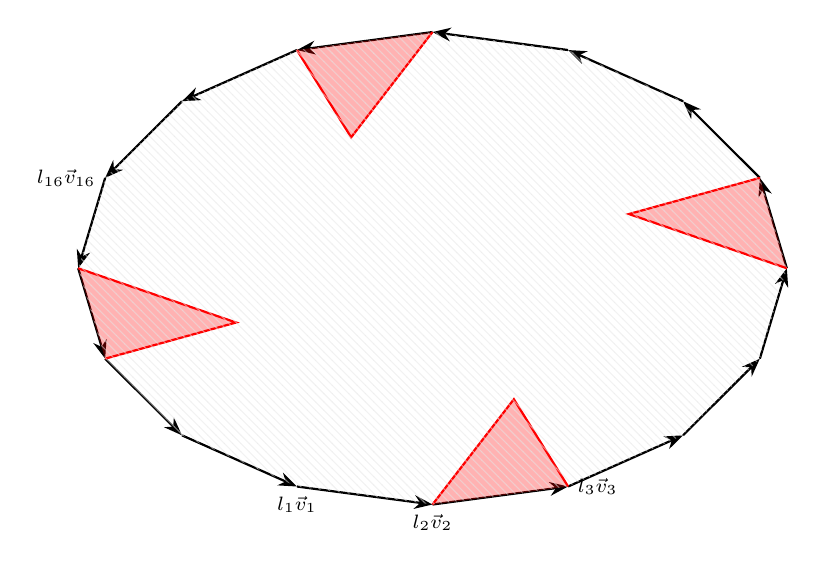
\begin{tikzpicture}[scale=3]
    % Define the 16 vertices of a squashed 16-gon
    \foreach \i in {0,1,...,15} {
        \coordinate (V\i) at ({1.5*cos(\i*22.5)}, {sin(\i*22.5)});
    }

    % Draw the directed edges
    \foreach \i in {0,1,...,15} {
        \pgfmathsetmacro{\next}{mod(\i+1, 16)}
        \draw[thick, -{Stealth}] (V\i) -- (V\next);
    }

    % 4 Red Surgery Triangles (pointing inwards)
    \foreach \i in {1, 5, 9, 13} {
        \pgfmathsetmacro{\prev}{mod(\i-1, 16)}
        \pgfmathsetmacro{\next}{mod(\i+1, 16)}
        \fill[red, opacity=0.3] (V\i) -- ($(V\i)!0.4!(0,0)$) -- (V\prev) -- cycle;
        \draw[red, thick] (V\i) -- ($(V\i)!0.4!(0,0)$) -- (V\prev);
    }

    % Labels for edges
    \node[font=\scriptsize, below] at (V11) {$l_1 \vec{v}_1$};
    \node[font=\scriptsize, below] at (V12) {$l_2 \vec{v}_2$};
    \node[font=\scriptsize, right] at (V13) {$l_3 \vec{v}_3$};
    \node[font=\scriptsize, left] at (V7) {$l_{16} \vec{v}_{16}$};

    % Central area hatching
    \begin{scope}
        \clip (V0) -- (V1) -- (V2) -- (V3) -- (V4) -- (V5) -- (V6) -- (V7) -- (V8) -- (V9) -- (V10) -- (V11) -- (V12) -- (V13) -- (V14) -- (V15) -- cycle;
        \fill[pattern=north west lines, pattern color=gray!20, opacity=0.5] (-2,-2) rectangle (2,2);
    \end{scope}

\end{tikzpicture}

\end{document}
